% Methodology section

\subsection{Operads}

A large class of mathematical theories consists of three ingredients:
\begin{enumerate}
  \item A collection of objects.
  \item A collection of morphisms between these objects.
  \item A notion of composition of these morphisms.
\end{enumerate}

The most well-known example of this pattern is arithmetic, where the objects are numbers, the morphisms are functions (addition, multiplication, etc.), and the composition is the usual function composition. All fields such as real numbers, complex numbers, and vector spaces can be described in this way.

As we go up the hierarchy of mathematics, we find more and more examples of this pattern. For example, in topology, the objects are topological spaces, the morphisms are continuous functions, and the composition is the usual function composition. Groups and family (magma, monoid, group, ring, field) are also examples of this pattern. Category theory is a generalization of this pattern, where the objects are categories, the morphisms are functors, and the composition is the usual functor composition.

Operads are a generalization of this pattern, where the objects are operations, the morphisms are operations of different arities, and the composition is a more general form of function composition. Operads provide a framework for studying algebraic structures that arise in various areas of mathematics, including topology, algebra, and category theory.

Operads consists of:

\begin{enumerate}
  \item A collection of operations of different arities.
  \item A notion of composition of these operations.
  \item The composition operations obey certain conditions - associativity and unitality.
\end{enumerate}

\subsubsection{Formal Definition}
\\

Consider a set $\mathbb{X}$, and an integer $n \in \mathbb{N}$.

An Operad, $\mathbb{P}$, is defined as a set of n-ary operations, where each operation $f$ has the signature $\mathbb{X}^n \to \mathbb{X}$:

\begin{equation}
  \mathbb{P}(n) = \{f: \mathbb{X}^n \to \mathbb{X}\}
\end{equation}

where $\mathbb{X}^n$ is the cartesian product of $\mathbb{X}$ with itself $n$ times, i.e.

\begin{equation}
  \mathbb{X}^n = \mathbb{X} \times \mathbb{X} \times \ldots \times \mathbb{X}
\end{equation}

i.e. all of these functions $f$ take in $n$ arguments from $\mathbb{X}$ and return a single element from $\mathbb{X}$.

\begin{figure}[h]
\centering
    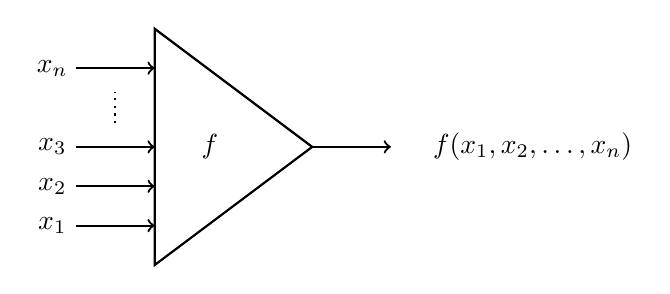
\begin{tikzpicture}
        % Draw the triangle with vertical left edge
        \draw[thick, fill=white] (0,0) -- (0,3) -- (2,1.5) -- cycle;

        % Draw input arrows
        \draw[->, thick] (-1,0.5) -- (0,0.5);
        \draw[->, thick] (-1,1) -- (0,1);
        \draw[->, thick] (-1,1.5) -- (0,1.5);
        \draw[dotted, thick] (-0.5,1.8) -- (-0.5,2.2);
        \draw[->, thick] (-1,2.5) -- (0,2.5);

        % Draw output arrow
        \draw[->, thick] (2,1.5) -- (3,1.5);

        % Add labels
        \node at (0.7,1.5) {$f$};
        \node at (-1.3,0.5) {$x_1$};
        \node at (-1.3,1) {$x_2$};
        \node at (-1.3,1.5) {$x_3$};
        \node at (4.8,1.5) {$f(x_1,x_2,\ldots,x_n)$};
        \node at (-1.3,2.5) {$x_n$};
    \end{tikzpicture}
\end{figure}

If we have a bunch of these sets of functions $\mathbb{P}(k_i)$ for each $k_i \in \mathbb{N}$, then we can define a composition operation $\circ$ for these operations as follows:

Let $f_i \in \mathbb{P}(k_i)$ be an operation that takes in $k_i$ arguments from $\mathbb{X}$ and returns a single element from $\mathbb{X}$. We can take n numbers of such operations and use their outputs as inputs to another operation $f \in \mathbb{P}(n)$, which takes in $n$ arguments from $\mathbb{X}$ and returns a single element from $\mathbb{X}$. The composition operation $\circ$ is defined as:

\begin{equation}
    \mathbb{P}(n) \times ( \mathbb{P}(k_1) \times \mathbb{P}(k_2) \times \ldots \times \mathbb{P}(k_n) ) \to \mathbb{P}(k_1 + k_2 + \ldots + k_n)
\end{equation}

\begin{equation}
    f, (f_1, f_2, \ldots, f_n) \mapsto f \circ (f_1, f_2, \ldots, f_n)
\end{equation}

where $f \circ (f_1, f_2, \ldots, f_n) \in \mathbb{P}(k_1 + k_2 + \ldots + k_n)$ is defined as the following diagram:

\begin{figure}[h]
\centering
\begin{tikzpicture}[scale=0.9]
    % Main operation triangle
    \draw[thick, fill=white] (0,0) -- (0,5.5) -- (4,2.75) -- cycle;
    \node at (1.5,2.75) {$f$};

    % First sub-operation triangle
    \draw[thick, fill=white] (-5,0) -- (-5,1.5) -- (-3,0.75) -- cycle;
    \node at (-4.3,0.75) {$f_1$};

    % Second sub-operation triangle
    \draw[thick, fill=white] (-5,2) -- (-5,3.5) -- (-3,2.75) -- cycle;
    \node at (-4.3,2.75) {$f_2$};

    % Third sub-operation triangle (with dotted line indicating more)
    \draw[thick, fill=white] (-5,4) -- (-5,5.5) -- (-3,4.75) -- cycle;
    \node at (-4.3,4.75) {$f_n$};

    % Dotted line between second and third triangles
    \draw[dotted, thick] (-4,3.7) -- (-4,4);

    % Input arrows for first sub-operation
    \draw[->, thick] (-7,0.25) -- (-5,0.25);
    \draw[->, thick] (-7,0.75) -- (-5,0.75);
    \draw[->, thick] (-7,1.25) -- (-5,1.25);
    \node at (-8.4,0.25) {$x_1}$};
    \node at (-8.4,0.75) {$\ldots$};
    \node at (-8.4,1.25) {$x_{k_1}$};

    % Input arrows for second sub-operation
    \draw[->, thick] (-7,2.25) -- (-5,2.25);
    \draw[->, thick] (-7,2.75) -- (-5,2.75);
    \draw[->, thick] (-7,3.25) -- (-5,3.25);
    \node at (-8.4,2.25) {$x_{k_1+1}}$};
    \node at (-8.4,2.75) {$\ldots$};
    \node at (-8.4,3.25) {$x_{k_1+k_2}$};

    % Input arrows for third sub-operation
    \draw[->, thick] (-7,4.25) -- (-5,4.25);
    \draw[->, thick] (-7,4.75) -- (-5,4.75);
    \draw[->, thick] (-7,5.25) -- (-5,5.25);
    \node at (-8.4,4.25) {$x_{k_1+...+k_{n-1}+1}$};
    \node at (-8.4,4.75) {$\ldots$};
    \node at (-8.4,5.25) {$x_{k_1+...+k_{n-1}+k_n}$};

    % Connecting arrows from sub-operations to main operation
    \draw[->, thick] (-3,0.75) -- (0,0.75);
    \draw[->, thick] (-3,2.75) -- (0,2.75);
    \draw[->, thick] (-3,4.75) -- (0,4.75);

    % Output arrow
    \draw[->, thick] (4,2.75) -- (6,2.75);

    % Final output label
    \node at (6,3.5) {$f \circ (f_1, f_2, \ldots, f_n)$};

    % Dotted lines to indicate more inputs for each sub-operation
    \draw[dotted, thick] (-6,1) -- (-6,1.1);
    \draw[dotted, thick] (-6,3) -- (-6,3.1);
    \draw[dotted, thick] (-6,4.5) -- (-6,4.6);

\end{tikzpicture}
\caption{Operadic composition showing how multiple operations $f_1, f_2, \ldots, f_n$ with arities $k_1, k_2, \ldots, k_n$ can be composed with an operation $f$ of arity $n$ to form a new operation of arity $k_1 + k_2 + \ldots + k_n$.}
\label{fig:operadic-composition}
\end{figure}

Associativity of this composition for Operads works as follows:

\begin{figure}[h]
\centering
    \begin{tikzpicture}[grow'=up]
        \begin{scope}[xshift=-5cm]
            \node {(ab)c}
            child {
                node {ab}
                child {
                    node {a}
                }
                child {
                    node {b}
                }
            }
            child{
                node {c}
            };
        \end{scope}
        \begin{scope}[xshift=0cm]
            \node {(ab)c}
            child{
                node {a}
            }
            child {
                node {bc}
                    child {
                node {b}
                }
                child {
                    node {c}
                }
            };
        \end{scope}
        \begin{scope}[xshift=5cm]
            \node {abc}
            child{
                node {a}
            }
            child {
                node {b}
            }
            child {
                node {c}
            };
        \end{scope}
    \end{tikzpicture}
    \caption{Associativity of operadic composition of arity 3}
\end{figure}

\begin{figure}[h]
\centering
\begin{tikzpicture}[grow'=up, level distance=1.5cm, sibling distance=2cm]
    % First tree: ((ab)c)d
    \begin{scope}[xshift=-10cm]
        \node {((ab)c)d}
        child {
            node {(ab)c}
            child {
                node {ab}
                child {
                    node {a}
                }
                child {
                    node {b}
                }
            }
            child {
                node {c}
            }
        }
        child {
            node {d}
        };
    \end{scope}

    % Second tree: (a(bc))d
    \begin{scope}[xshift=-5cm]
        \node {(a(bc))d}
        child {
            node {a(bc)}
            child {
                node {a}
            }
            child {
                node {bc}
                child {
                    node {b}
                }
                child {
                    node {c}
                }
            }
        }
        child {
            node {d}
        };
    \end{scope}

    % Third tree: (ab)(cd)
    \begin{scope}[yshift=6cm, xshift=0cm]
        \node {(ab)(cd)}
        child {
            node {ab}
            child {
                node {a}
            }
            child {
                node {b}
            }
        }
        child {
            node {cd}
            child {
                node {c}
            }
            child {
                node {d}
            }
        };
    \end{scope}

    % Fourth tree: a((bc)d)
    \begin{scope}[yshift=6cm, xshift=-10cm]
        \node {a((bc)d)}
        child {
            node {a}
        }
        child {
            node {(bc)d}
            child {
                node {bc}
                child {
                    node {b}
                }
                child {
                    node {c}
                }
            }
            child {
                node {d}
            }
        };
    \end{scope}

    % Fifth tree: a(b(cd))
    \begin{scope}[yshift=6cm, xshift=-5cm]
        \node {a(b(cd))}
        child {
            node {a}
        }
        child {
            node {b(cd)}
            child {
                node {b}
            }
            child {
                node {cd}
                child {
                    node {c}
                }
                child {
                    node {d}
                }
            }
        };
    \end{scope}

    \begin{scope}
        \node {abcd}
        child {
            node {a}
        }
        child {
            node {b}
        }
        child {
            node {c}
        }
        child {
            node {d}
        };
    \end{scope}

\end{tikzpicture}
\caption{Associativity of operadic composition of arity 4}
\label{fig:arity-4-associativity}
\end{figure}

This composition operation $\circ$ satisfies the following properties:

\begin{itemize}
  \item \textbf{Associativity}: For all $f \in \mathbb{P}(n)$, $g \in \mathbb{P}(k_1)$, $h \in \mathbb{P}(k_2)$, and $i \in \mathbb{P}(k_3)$, we have:

  \begin{equation}
    f \circ (g \circ (h, i)) = (f \circ (g, h)) \circ i
  \end{equation}

  \item \textbf{Unitality}: For all $f \in \mathbb{P}(n)$, we have:

  \begin{equation}
    f \circ (\text{id}_{k_1}, \text{id}_{k_2}, \ldots, \text{id}_{k_n}) = f
  \end{equation}

  where $\text{id}_k$ is the identity function on $\mathbb{X}^k$.
\end{itemize}

Symmetry is not required for operads, but it can be added to form symmetric operads. The symmetry condition is:

\begin{equation}
  f \circ (g_1, g_2, \ldots, g_n) = f \circ (g_{\sigma(1)}, g_{\sigma(2)}, \ldots, g_{\sigma(n)})
\end{equation}

where $\sigma$ is a permutation of the set $\{1, 2, \ldots, n\}$ or $\sigma \in S_n$ and $g_{\sigma(i)}$ is the $\sigma(i)$-th element of the original sequence, i.e., the permutation $\sigma$ permutes the order of operations used as inputs to $f$.

\subsection{T-operads}

Operads, as defined above, are based on operations without any structural restrictions, e.g., if one would want to model systems where operations must respect specific input configurations, say restrictions on the types of inputs, or arity of the operations, then one would need to define a set of operations that are not just arbitrary functions but have some structure. This is where T-operads come in. T-operads extend the concept of operads by parameterizing the structure of operations through a monad T, which encodes the shape or type of input configurations and the rules for their composition, allowing for a more flexible and generalized framework that can accommodate various algebraic and categorical structures beyond simple arity-based operations.

\textbf{Formal Definition}
\\

A T-operad generalizes the concept of an operad by using a monad T on a category to determine the allowable shapes or configurations of inputs for operations. It consists of:

\begin{enumerate}
  \item A set of objects (often thought of as "colors" or "types"), denoted as Obj($\mathcal{P}$).
  \item For each shape $t \in T(X)$, where $X \subseteq$ Obj($\mathcal{P}$) is a set of input objects, and for each output object $b \in$ Obj($\mathcal{P}$), a set of operations $\mathcal{P}(t; b)$.
  \item A composition operation that respects the structure defined by the monad T.
  \item Identity operations for each object, consistent with the unit of the monad T.
\end{enumerate}

More formally, let $\mathcal{C}$ be a category (e.g., the category of sets), and let T be a monad on $\mathcal{C}$. A T-operad $\mathcal{P}$ assigns to each shape $t \in T(X)$, where $X$ is a set of input objects, and each output object $b$, a set (or object in $\mathcal{C}$) of operations $\mathcal{P}(t; b)$ that take inputs shaped by $t$ and produce an output of type $b$:

\begin{equation}
  \mathcal{P}(t; b) = \{\text{operations with input shape } t \text{ and output } b\}
\end{equation}

In the context of sets, if we think of $X$ as a set of types or objects, and $t \in T(X)$ as a structured configuration of inputs (e.g., a list, tree, or graph built from $X$), then $\mathcal{P}(t; b)$ represents operations that transform inputs configured as $t$ into an output of type $b$.

\begin{figure}[h]
\centering
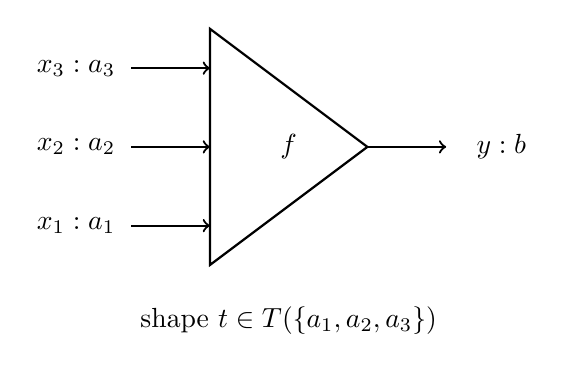
\begin{tikzpicture}
    % Draw the triangle with vertical left edge
    \draw[thick, fill=white] (0,0) -- (0,3) -- (2,1.5) -- cycle;

    % Draw input arrows
    \draw[->, thick] (-1,0.5) -- (0,0.5);
    \draw[->, thick] (-1,1.5) -- (0,1.5);
    \draw[->, thick] (-1,2.5) -- (0,2.5);

    % Draw output arrow
    \draw[->, thick] (2,1.5) -- (3,1.5);

    % Add labels
    \node at (1,1.5) {$f$};
    \node at (-1.7,0.5) {$x_1: a_1$};
    \node at (-1.7,1.5) {$x_2: a_2$};
    \node at (-1.7,2.5) {$x_3: a_3$};
    \node at (3.7,1.5) {$y: b$};
    \node at (1,-0.7) {shape $t \in T(\{a_1, a_2, a_3\})$};
\end{tikzpicture}
\caption{A typed operation $f \in \mathcal{P}(t; b)$ taking inputs shaped by $t \in T(\{a_1, a_2, a_3\})$ and producing an output of type $b$.}
\label{fig:shaped-operation}
\end{figure}

The composition operation must respect the structure defined by the monad T. Given operations:
\begin{itemize}
  \item $f \in \mathcal{P}(t; b)$, where $t \in T(X)$ for some set of input objects $X = \{a_1, a_2, \ldots, a_n\}$,
  \item $g_1 \in \mathcal{P}(s_1; a_1)$, where $s_1 \in T(Y_1)$ for some set $Y_1$,
  \item $g_2 \in \mathcal{P}(s_2; a_2)$, where $s_2 \in T(Y_2)$ for some set $Y_2$,
  \item $\ldots$
  \item $g_n \in \mathcal{P}(s_n; a_n)$, where $s_n \in T(Y_n)$ for some set $Y_n$,
\end{itemize}

The composition $f \circ (g_1, g_2, \ldots, g_n)$ is defined using the monad's multiplication $\mu: T^2 \to T$, which combines the shapes $s_1, s_2, \ldots, s_n$ into a new shape compatible with $t$. The resulting operation has inputs shaped by a new configuration in $T(Y_1 \cup Y_2 \cup \ldots \cup Y_n)$ and output type $b$:

\begin{equation}
  f \circ (g_1, g_2, \ldots, g_n) \in \mathcal{P}(\mu(t; s_1, s_2, \ldots, s_n); b)
\end{equation}

where $\mu(t; s_1, s_2, \ldots, s_n)$ represents the combined shape obtained through the monad's multiplication.

\begin{figure}[h]
\centering
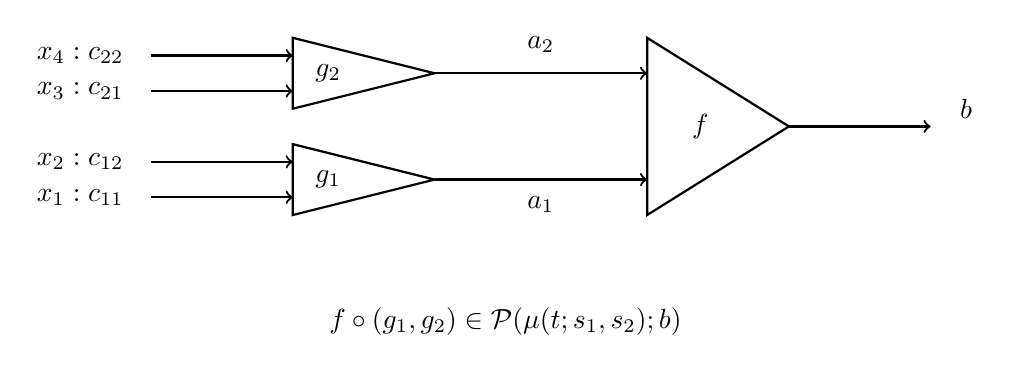
\begin{tikzpicture}[scale=0.9]
    % Main operation triangle
    \draw[thick, fill=white] (0,0) -- (0,2.5) -- (2,1.25) -- cycle;
    \node at (0.75,1.25) {$f$};

    % First sub-operation triangle
    \draw[thick, fill=white] (-5,0) -- (-5,1) -- (-3,0.5) -- cycle;
    \node at (-4.5,0.5) {$g_1$};

    % Second sub-operation triangle
    \draw[thick, fill=white] (-5,1.5) -- (-5,2.5) -- (-3,2) -- cycle;
    \node at (-4.5,2) {$g_2$};

    % Input arrows for first sub-operation
    \draw[->, thick] (-7,0.25) -- (-5,0.25);
    \draw[->, thick] (-7,0.75) -- (-5,0.75);
    \node at (-8,0.25) {$x_1: c_{11}$};
    \node at (-8,0.75) {$x_2: c_{12}$};

    % Input arrows for second sub-operation
    \draw[->, thick] (-7,1.75) -- (-5,1.75);
    \draw[->, thick] (-7,2.25) -- (-5,2.25);
    \node at (-8,1.75) {$x_3: c_{21}$};
    \node at (-8,2.25) {$x_4: c_{22}$};

    % Connecting arrows from sub-operations to main operation
    \draw[->, thick] (-3,0.5) -- (0,0.5);
    \node at (-1.5,0.15) {$a_1$};
    \draw[->, thick] (-3,2) -- (0,2);
    \node at (-1.5,2.4) {$a_2$};

    % Output arrow
    \draw[->, thick] (2,1.25) -- (4,1.25);
    \node at (4.5,1.5) {$b$};

    % Final composition label
    \node at (-2,-1.5) {$f \circ (g_1, g_2) \in \mathcal{P}(\mu(t; s_1, s_2); b)$};

\end{tikzpicture}
\caption{Composition in a T-operad showing how the output types of $g_1$ and $g_2$ must match the input objects required by the shape $t \in T(\{a_1, a_2\})$ of $f$, with shapes combined via the monad's multiplication $\mu$.}
\label{fig:t-operadic-composition}
\end{figure}

The composition operation satisfies properties of associativity and unitality, which are ensured by the monadic structure of T (i.e., the associativity of the monad's multiplication $\mu$ and the unitality provided by the monad's unit $\eta$).

A T-Operad can be used to model any mathematical structure that can be described by a monad, such as:
\begin{itemize}
    \item Algebraic structures (e.g., groups, rings, modules)
    \item Topological structures (e.g., simplicial complexes, CW-complexes)
    \item Categorical structures (e.g., categories, functors)
    \item Combinatorial structures (e.g., trees, graphs)
    \item Geometric structures (e.g., manifolds, polyhedra)
    \item Logical structures (e.g., propositional logic, predicate logic)
\end{itemize}

This gives them the power and flexibility to model a wide range of mathematical phenomena, including those that arise in complex systems, such as hierarchical organization, modularity, and self-similarity.

